\subsection{GUI Implementation}
\label{ssec:GUI-implement}

Initially the \acrfull{GUI} was to be implemented using JavaFX \cite{javafx}, and any MATLAB additions would be linked in, however it became apparent that it is possible to create \acrshort{GUI}s easily within MATLAB itself. GUIDE \cite{guide} is MATLAB`s Application development environment where you can either build using purely drag-and-drop techniques, program the application like normal in the editor, or both.

The combination of both the drag-and-drop environment, and manually programming via the editor was undertaken during this project, to allow a greater amount of freedom and flexibility. Drag-and-drop was leveraged to style the \acrshort{GUI} and the editor was used to program the functionality in the back-end and link in the \Gls{Congealing} and Fuzzy Entropy algorithms.

The design process, including wireframes, of the \acrshort{GUI} can be seen in the earlier Subsection \ref{sssec:gui-design}.

\begin{figure}[H]
  \center
  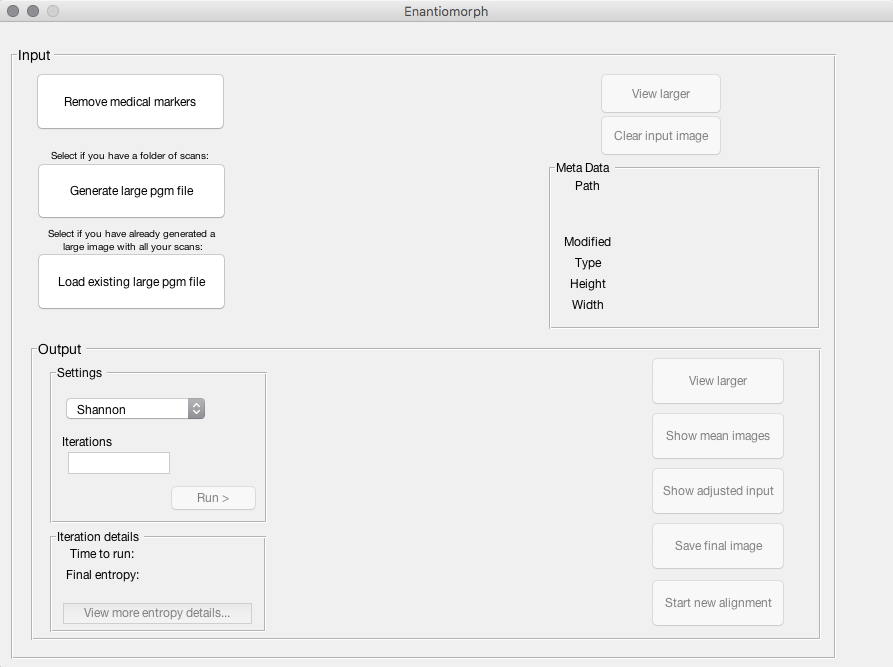
\includegraphics[scale=0.5]{Chapter2/software-img/final_gui.png}
  \caption{The main Graphical User Interface (GUI)}
  \label{fig:final_gui_pic}
\end{figure}

Figure \ref{fig:final_gui_pic} gives a snapshot of the final application implemented for users to align their images.

\vspace{2cm}

\noindent \textbf{\acrshort{GUI} breakdown: }

\noindent \textbf{ A: } Users can remove medical markers (or any other artefacts) from their mammographic images prior to creating the image to be congealed. This in itself is a separate \acrshort{GUI}, which will be covered later in the Section.

\noindent \textbf{ B: } After removing medical markers, the user can go on to `generate' a large pgm file, which will contain all the mammographic images they wish to align. This will then proceed to load the large pgm into the application. If the user has already generated one of these images, they can simply choose to load it instead.

\noindent \textbf{ C: } Once the image is loaded in, it will be displayed here.

\noindent \textbf{ D: } Should they wish, the user can view their input image larger, or clear the image should they upload the wrong file.

\noindent \textbf{ E: } Metadata about the image is displayed here.

\noindent \textbf{ F: } The user can select the image alignment metric from the drop-down menu, and enter the number of iterations they wish to perform. Pressing the `Run' button will start the \Gls{Congealing} algorithm, and the user will see an egg-timer/pinwheel to signify it is running.

\noindent \textbf{ G: } Once the images have been aligned, the final average image will be displayed here.

\noindent \textbf{ H: } Information about how long the congealing process took, and the final entropy value will be displayed here. Users can choose to view a graph detailing the reduction in entropy over each iteration using the `View more entropy details...' button should they wish.

\noindent \textbf{ I: } These buttons allow the user to choose what to do next. They can either view the final mean image larger, view the mean images for each iteration run, see how the input images have adjusted to fit in the final mean image, save the final mean image or clear the application ready to run a new alignment.

\begin{figure}[H]
  \center
  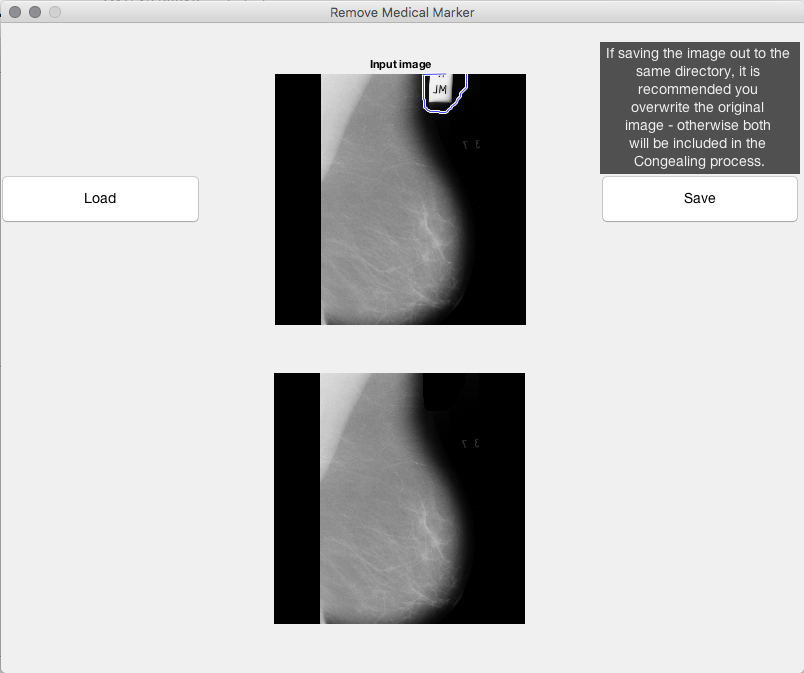
\includegraphics[scale=0.5]{Chapter2/software-img/removeMarker.png}
  \caption{The Graphical User Interface (GUI) for removing medical markers}
  \label{fig:medical_gui}
\end{figure}

Figure \ref{fig:medical_gui} details the \acrshort{GUI} in which the user can remove medical markers/other artefacts. This simple user interface allows them to simply:
\begin{itemize}
  \item Load in the image of their choice
  \item A pop-up (not pictured) gives them instructions on how to draw on the image
  \item The user then draws around the area they would like to remove
  \item The final image is displayed in the second image
  \item The user can save the image back out, overwriting the original if they wish
\end{itemize}

Once all the unnecessary markers or artefacts have been removed, the user can close the \acrshort{GUI} and be returned to the main application.
